%%% Содержимое слайдов

\frame[plain]{\titlepage} % Титульный слайд

%-------------------------------------------------------------------------------

\section{Разработка виртуальной инфраструктуры для реализации облачных услуг}

\begin{frame}
\frametitle{\insertsection}
Требования:
\begin{itemize}
	\item устранение единых точек отказа %(резервные линки, RAID)
	\item защита от недоброжелателей %(DDoS, флуд)
	\item \textbf{использование свободного ПО по возможности}
	\item документирование
	\item автоматизация
	\item разработка эффективных тарифных планов хостинга
	\item использование в бизнесе
\end{itemize}
\end{frame}

\begin{frame}
\frametitle{\insertsection}
Возможности:
\begin{itemize}
	\item весьма ограниченный бюджет
	\item всего один админ, он же архитектор (некрасиво звучит этот пункт)
	\item отсутствие опыта работы с виртуализацией
	\item желание что-то построить
	\item ??? что-то еще упустил ???
\end{itemize}
\end{frame}

%-------------------------------------------------------------------------------

\section{Общая схема инфраструктуры}

\begin{frame}
\frametitle{\insertsection}
\begin{figure}[h]
	\begin{center}
		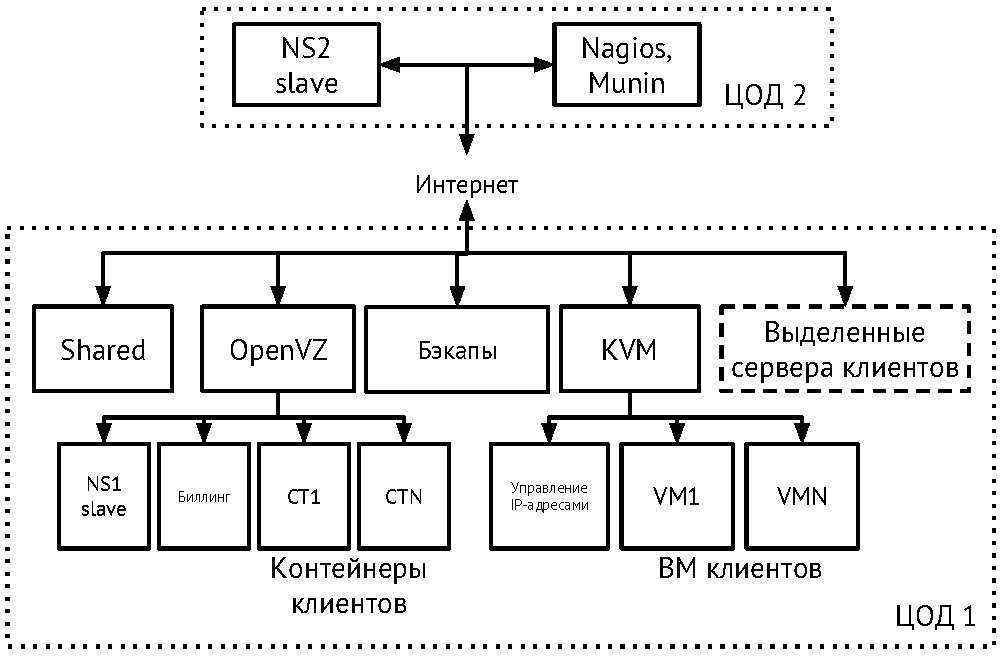
\includegraphics[width=\linewidth]{infrast-scheme}
	 \end{center}
\end{figure}
\end{frame}

%-------------------------------------------------------------------------------

\section{Используемое свободное ПО !(не очень заголовок)}

\begin{frame}
\frametitle{\insertsection}
\begin{itemize}
	\item ОС Linux
	\item мониторинг
	\item виртуализация
	\item автоматизированное управление конфигурациями
	\item скрипты, много скриптов
	\item стандартный стек хостинга
	\item вирусы и malware на хостинге
	\item панели для пользователей виртуальных серверов
\end{itemize}
\end{frame}

%-------------------------------------------------------------------------------

\section{ОС}

\begin{frame}
\frametitle{\insertsection}
\framesubtitle{CentOS 7 (GPL)}
\begin{itemize}
	\item 494 из 500 крупнейших суперкомпьютеров работают на Linux
	\item изобилие серверного ПО
	\item поддержка 6-10 лет (обновление пакетов, исправление уязвимостей и багов)
	\item бесплатно
	\item простая сборка пакетов
	\item драйвера
	\item много документации
\end{itemize}
\end{frame}

%-------------------------------------------------------------------------------

\section{Мониторинг}

\begin{frame}
\frametitle{\insertsection}
\framesubtitle{Nagios → Icinga2 (GPLv2)}
\begin{figure}[h]
	\begin{center}
		\begin{multicols}{2}
		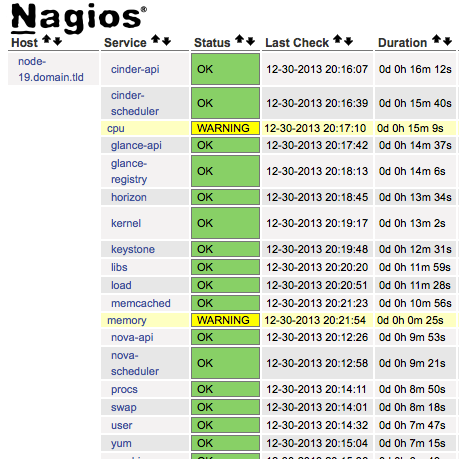
\includegraphics[width=\linewidth]{nagios} \pause \\
		\uncover<2->{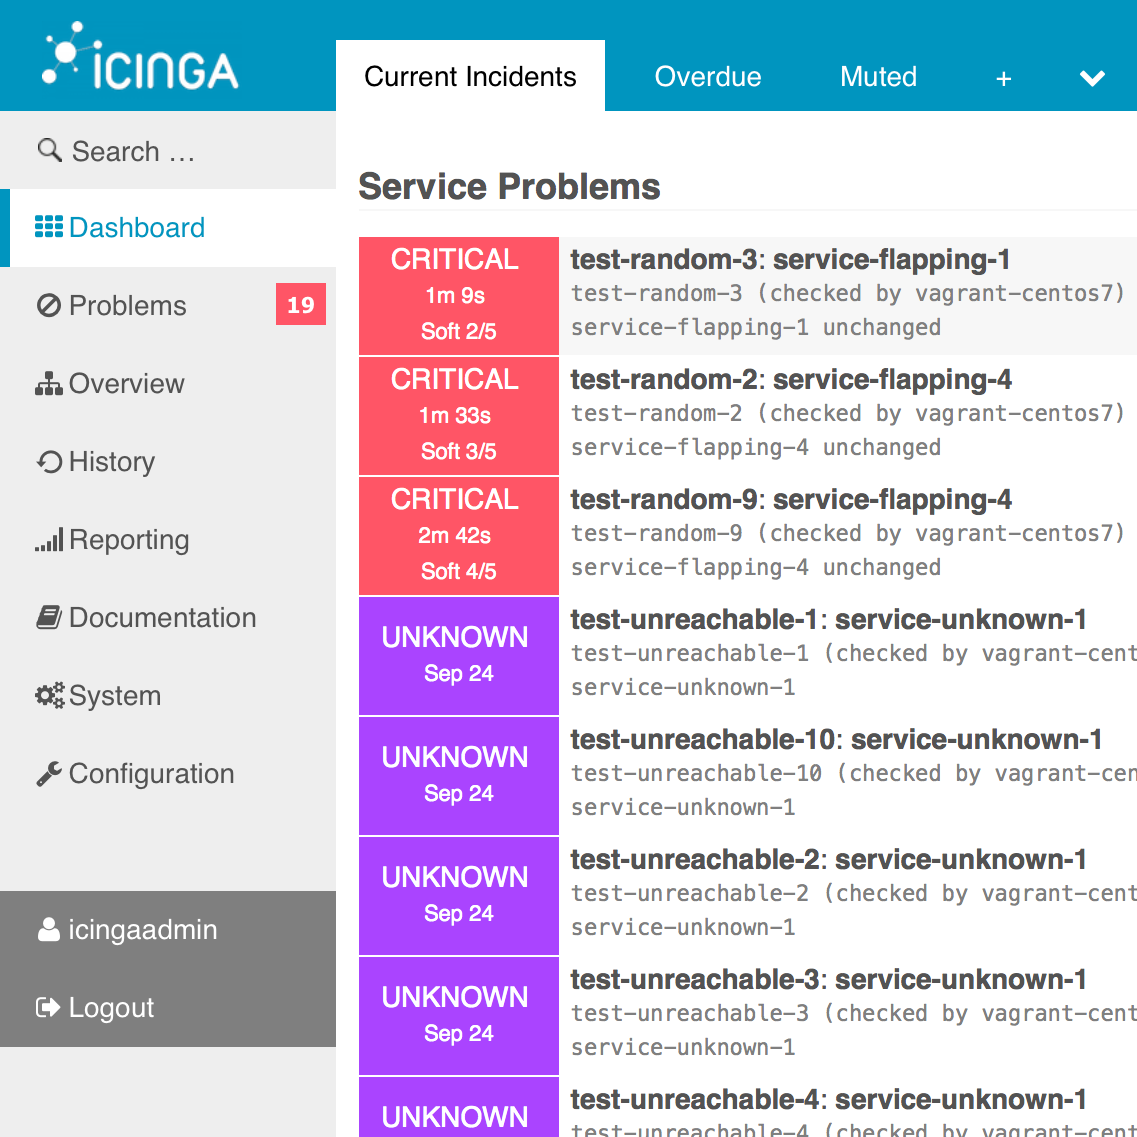
\includegraphics[width=\linewidth]{icinga2}}
		\end{multicols}
	 \end{center}
\end{figure}
\end{frame}

%-------------------------------------------------------------------------------

\section{Метрики}

\begin{frame}
\frametitle{\insertsection}
\framesubtitle{Munin (GPL)}
\begin{figure}[h]
	\begin{center}
		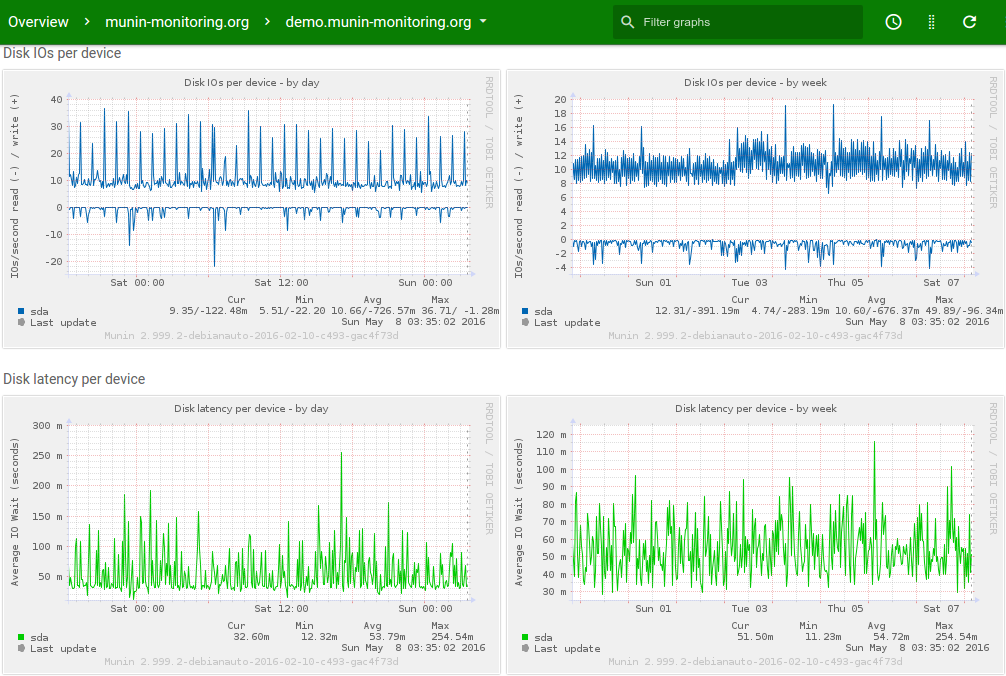
\includegraphics[width=\linewidth]{munin}
	 \end{center}
\end{figure}
\end{frame}

%-------------------------------------------------------------------------------

\section{Управление конфигурациями}

\begin{frame}
\frametitle{\insertsection}
\framesubtitle{Ansible (GPL) + git (GPLv2)}
\begin{figure}[h]
	\begin{center}
		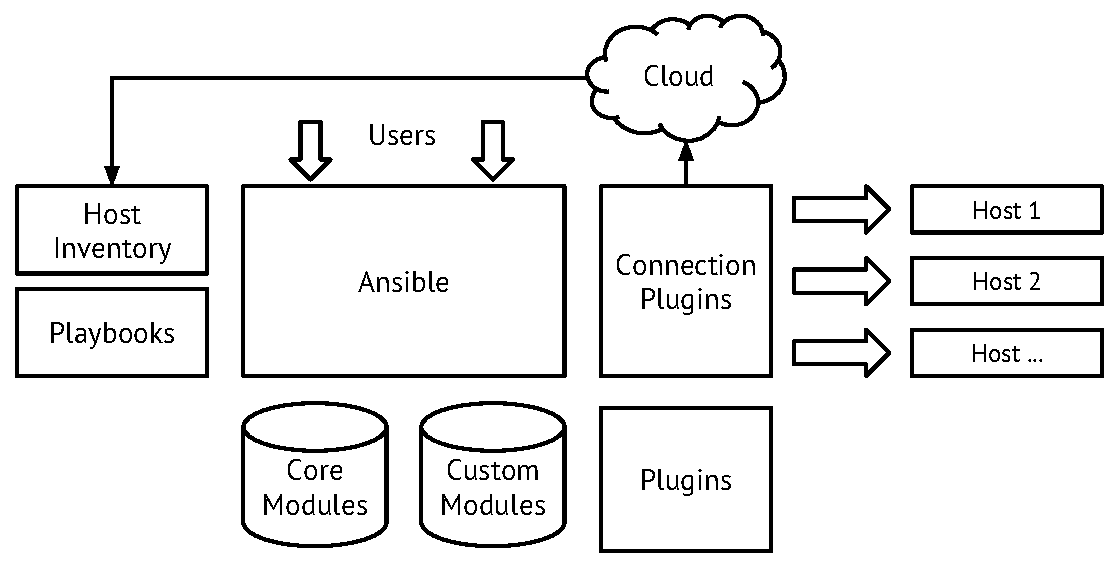
\includegraphics[width=\linewidth]{ansible}
	 \end{center}
\end{figure}
\end{frame}

%-------------------------------------------------------------------------------

\section{Виртуализация}

\begin{frame}
\frametitle{\insertsection}
\framesubtitle{OpenVZ (GPLv2) + KVM (GPL/LGPL)}
\begin{figure}[h]
	\begin{center}
		\begin{multicols}{2}
		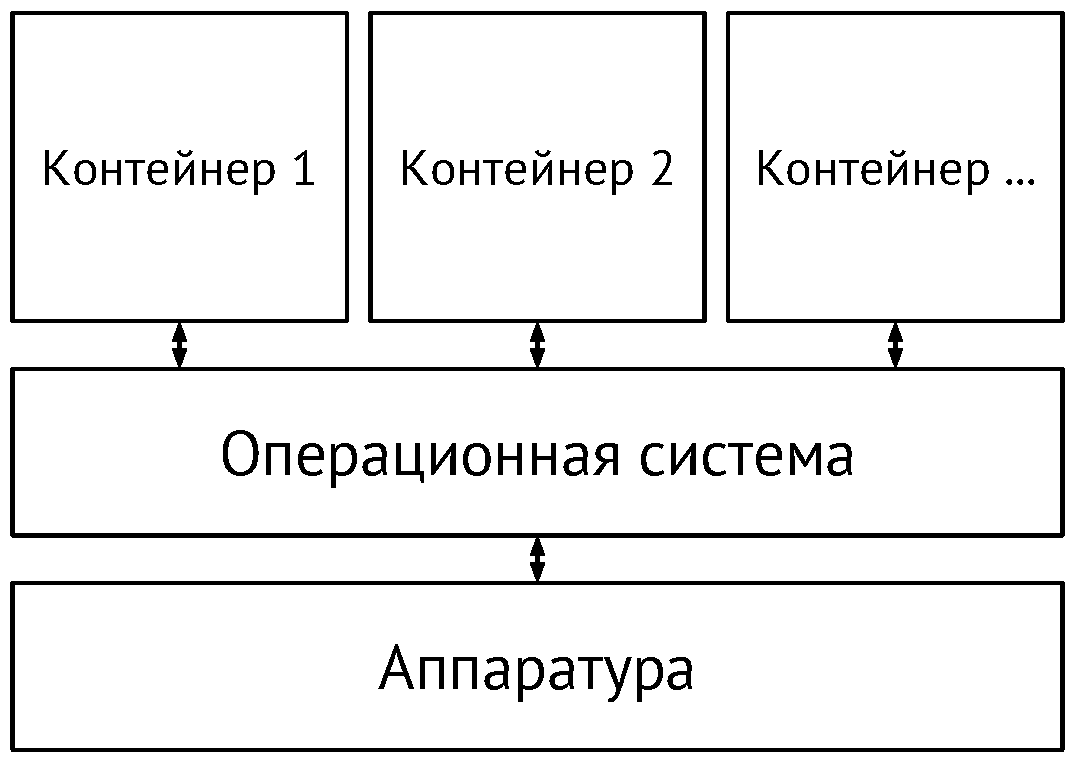
\includegraphics[width=\linewidth]{cont-virt} \\
		OpenVZ \pause \\
		\uncover<2->{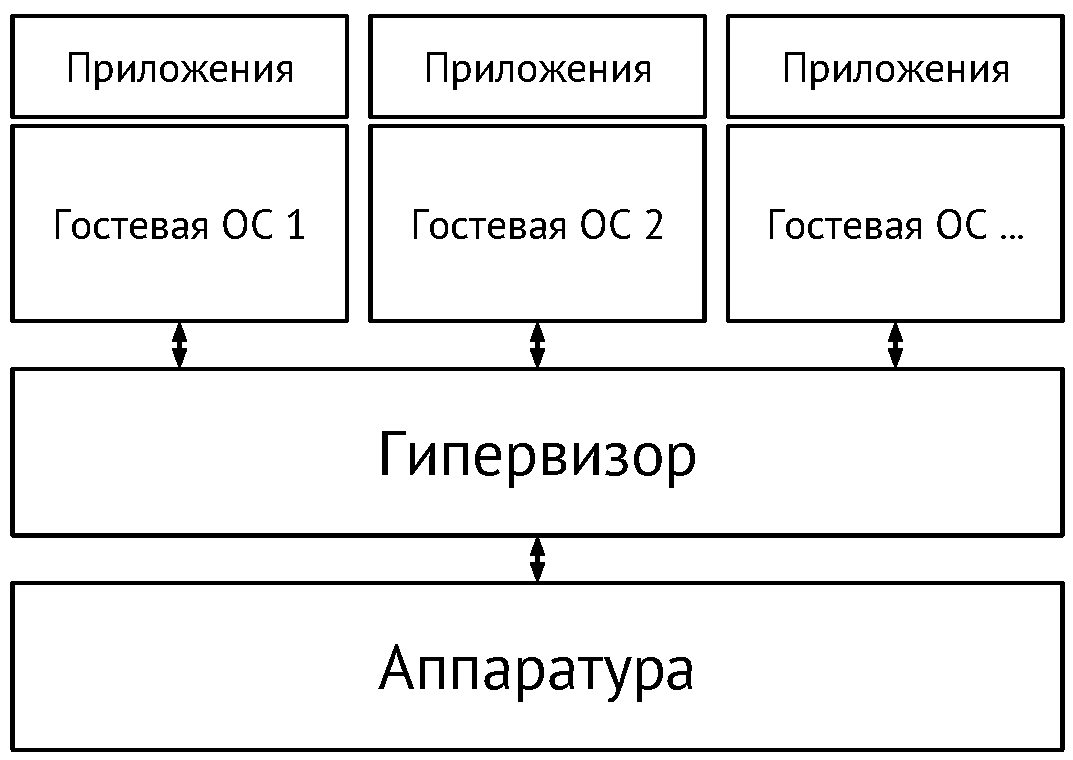
\includegraphics[width=\linewidth]{full-virt}}
		KVM
		\end{multicols}
	 \end{center}
	\end{figure}
\end{frame}

%-------------------------------------------------------------------------------

\section{Стек ПО для хостинга}

\begin{frame}
\frametitle{\insertsection}
\framesubtitle{LAMP+Nginx (GPL/Apache), exim+dovecot+spamassasin+roundcube (GPL/LGPL/MIT)}
\begin{figure}[h]
	\begin{center}
		\begin{multicols}{2}
		
\includegraphics[width=\linewidth]{lamp} \\
		
\includegraphics[width=\linewidth]{mail}
		\end{multicols}
	 \end{center}
	\end{figure}
\end{frame}

%-------------------------------------------------------------------------------

\section{Резервное копирование}

\begin{frame}
\frametitle{\insertsection}
\framesubtitle{rsync (GPL)}
\begin{figure}[h]
	\begin{center}
		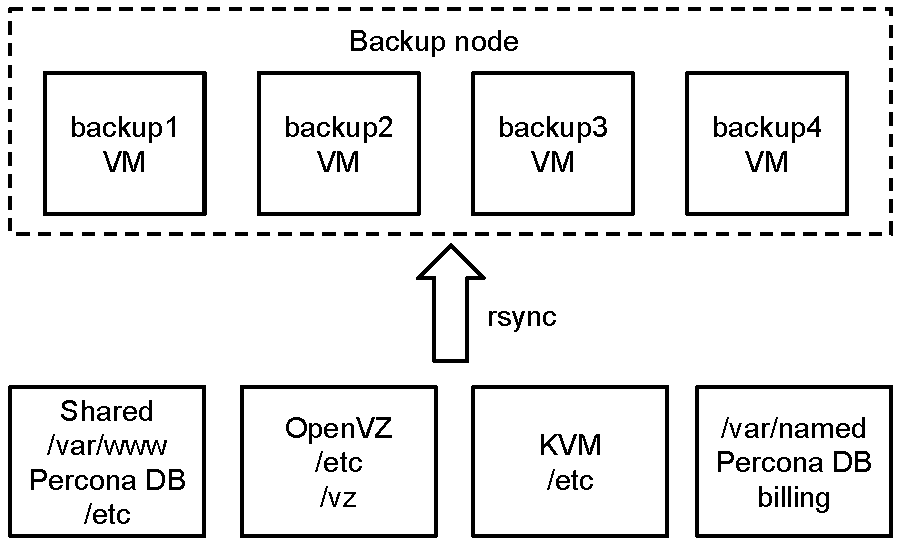
\includegraphics[width=\linewidth]{backup}
	 \end{center}
\end{figure}
\end{frame}

%-------------------------------------------------------------------------------

\section{Вирусы и вредоносы}

\begin{frame}
\frametitle{\insertsection}
\framesubtitle{Linux Malware Detect (GPL)}
Возможности:
\begin{itemize}
	\item обнаружение вредоносов по хэшу MD5
	\item отправка на rfxn.com подозрительных файлов для внесения в базу сигнатур
	\item выборочное сканирование путей
	\item exclude-файлы
	\item правила удаление инфицированных base64 и gzinflate вставок из файлов
	\item карантин
	\item возможность поиска по сигнатурам ClamAV
\end{itemize}
\end{frame}

%-------------------------------------------------------------------------------

\section{Защита сети}

\begin{frame}
\frametitle{\insertsection}
\framesubtitle{ddos-deflate (Artistic License) + IPTables/fail2ban/ipset (GPL)}
\begin{figure}[h]
	\begin{center}
		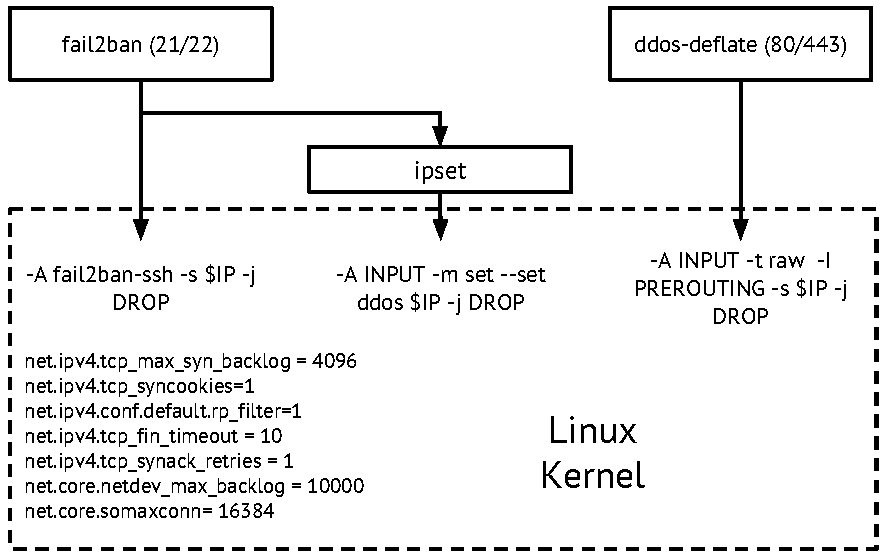
\includegraphics[width=\linewidth]{iptables}
	 \end{center}
\end{figure}
\end{frame}

%-------------------------------------------------------------------------------

\section{Панели управления для клиентов}

\begin{frame}
\frametitle{\insertsection}
\framesubtitle{Vesta Control Panel (GPLv3)}
\begin{figure}[h]
	\begin{center}
		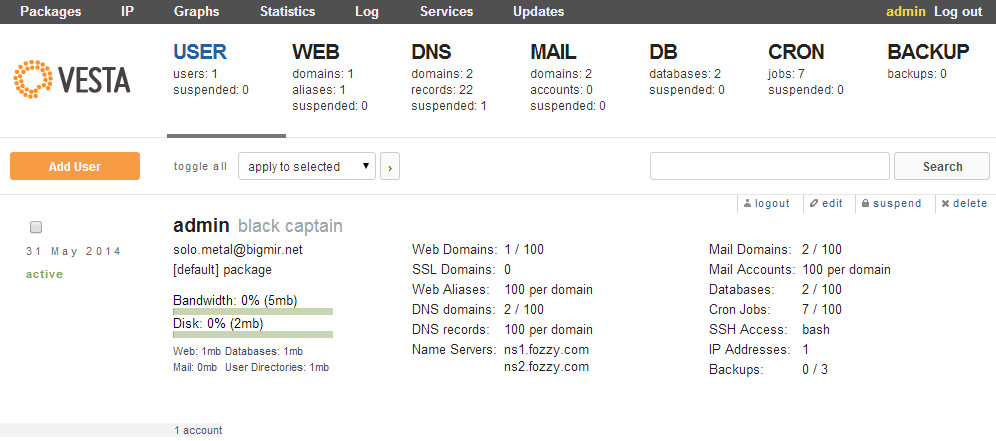
\includegraphics[width=\linewidth]{vesta}
	 \end{center}
\end{figure}
\end{frame}

%-------------------------------------------------------------------------------

\section{Коммерческие альтернативы}

\begin{frame}
\frametitle{\insertsection}
ОС:
\begin{itemize}
	\item RHEL 7 Standart --- \$900/год за 1 сервер
	\item SLES --- \$700/год за 1 сервер
\end{itemize}
Мониторинг:
\begin{itemize}
	\item Sensu --- \$2400/год за 100 серверов
	\item Opsview --- \$1870/год за 100 серверов
\end{itemize}
Виртуализация:
\begin{itemize}
	\item Virtuozzo --- \$6200/год за 100 контейнеров, 4 CPU
	\item VMWare vCenter Server --- \$1750/год, 1 CPU
\end{itemize}
Защита от вредоносного ПО:
\begin{itemize}
	\item Virusdie --- \$20/год за первый сайт, ~\$1/год за последующие сайты
\end{itemize}
\end{frame}

%-------------------------------------------------------------------------------

\section{Проекты в Open Source}

\begin{frame}
\frametitle{\insertsection}
\begin{itemize}
	\item openvz-tutorial (CC BY-SA 4.0): \href{https://github.com/Amet13/openvz-tutorial}{github.com/Amet13/openvz-tutorial}
	\item virtuozzo-tutorial (CC BY-SA 4.0): \href{https://github.com/Amet13/virtuozzo-tutorial}{github.com/Amet13/virtuozzo-tutorial}
	\item ddos-defalte (Artistic License 2.0): \href{https://github.com/Amet13/ddos-deflate}{github.com/Amet13/ddos-deflate}
	\item ansible-vz-wordpress (GNU GPLv3): \href{https://github.com/Amet13/ansible-vz-wordpress}{github.com/Amet13/ansible-vz-wordpress}
	\item icinga2-plugins-extra (GNU GPLv3): \href{https://github.com/Amet13/icinga2-plugins-extra}{github.com/Amet13/icinga2-plugins-extra}
	\item bachelor-diploma (CC BY-SA 4.0): \href{https://github.com/Amet13/bachelor-diploma}{github.com/Amet13/bachelor-diploma}
\end{itemize}
\end{frame}

%-------------------------------------------------------------------------------

\frame[plain]{\titlepage} % Титульный слайд
